% Chapter Template

\chapter{Results} % Main chapter title

\label{Chapter5} % Change X to a consecutive number; for referencing this chapter elsewhere, use \ref{ChapterX}

This section covers the results of the GNSS reception and GPS transmission experiments. Section \ref{sec:Res_GNSSReception} covers the attempts at receiving authentic GNSS
signals and accurately calculating a location. Section \ref{sec:Res_GPSTransmission} will cover the attempts and results of performing spoofing attacks on GPS receivers.
%----------------------------------------------------------------------------------------
%	SECTION 1
%----------------------------------------------------------------------------------------

\section{GNSS Reception} \label{sec:Res_GNSSReception}
Before testing the GPS transmission performance of the SDR, reception was tested, with less success. Three antenna setups were chosen each failing to lock and track the
satellites. A log linear, an omnidirectional and an active patch antenna were all used. The active antenna should have given best results since it includes amplifiers and
filters within the antenna module itself. The failure could be to do with the bias-t used to inject the 5V DC into the antenna, however testing with a multi-meter showed
that there was 5V on the RF+DC port of the Tee.

%----------------------------------------------------------------------------------------
%	SECTION 2
%----------------------------------------------------------------------------------------

\section{GPS Transmission} \label{sec:Res_GPSTransmission}
Experimentation was performed at the Tonsley campus of Flinders University, which has coordinates of $-35.007650, 138.572030$. At first it was decided to use the
centre of the Adelaide CBD as the coordinates for spoofing, that is $-34.5571732282, 138.3599516878$. Therefore it would be considered successful if the GPS receiver was to show
that the current location was in the CBD. This was extended to include other locations, Davis Station in Antarctica and the MAB at Flinders University Tonsley Campus with
coordinates of $-68.5762449235, 77.9696166515$ and $-35.00792163316667, 138.5715065625$ respectively.

Dynamic spoofing attacks were set to the road surrounding the MAB and around the CBD of Adelaide. All spoof attack dates were set to the same date, which was chosen to be
the 30th March 2021. This was arbitrary and only chosen since this was when official testing began.

\subsection{Meaconing Attack}
Since the GPS reception failed with the SDR, there was no way of performing a meaconing attack. Therefore, the only viable attack strategy was to generate a binary file
of the intended location. It would be ideal to perform this kind of attack in the future since this is the only basic attack type that can be used on the encrypted
military band.

\subsection{Spoofing Attack}
Once the workflow and hardware setup for the SDR was properly configured it was found that a smartphone was able to be spoofed.
When attempting to spoof devices in the wild, the Pixel XL smartphone was susceptible to attack while more modern smartphones that were tested were not susceptible. These
included the iPhone 12 Pro, Samsung Galaxy S10 and Google Pixel 3XL. The spoofing setup was not able to fool any of these devices. This could be down to software based
anti-spoofing algorithms that have been implemented including the usage of multiple constellations for position resolution.

\subsection{Static Spoofing}
\subsubsection{Tonsley MAB}
The grassed area outside of the Flinders University Tonsley campus was chosen as one of the points to spoof to. As mentioend above the desired coordinates that the receiver were
$-35.00792163316667, 138.5715065625$.

From Figure \ref{fig:MABStaticPosition} it can be seen that there are negative numbers, this is arbitrary and was included in order to give perspective as to which direction
the received position was wrong.

In this example the time to first fix was calculated as being 37 seconds. This is quite good for a cold start situation. During experimentation the time to first fix has
been variable between 30 seconds and 180 seconds. A trend has been the quicker the fix the better the overall accuracy of the spoofed location.

\begin{figure}[!h]
    \begin{centering}
        \includegraphics[width=14cm,keepaspectratio]{Figures/2021_3_30_static_MAB Carrier noise ratio.png}
        \caption{Carrier to noise ratio from unique SVIDs as broadcast by SDR and received by GPS receiver at MAB in Tonsley on 30th March 2021. Each SVID has been given a unique colour.}
        \label{fig:MABStaticCNo}
    \end{centering}
\end{figure}

\begin{figure}[!h]
    \begin{centering}
        \includegraphics[width=14cm,keepaspectratio]{Figures/2021_3_30_static_MAB Lat long position.png}
        \caption{Trace of latitude and longitude over time as interpreted from the GPS receiver with expected location noted with red dot}
        \label{fig:MABStaticCoord}
    \end{centering}
\end{figure}

\begin{figure}[!h]
    \begin{centering}
        \includegraphics[width=14cm,keepaspectratio]{Figures/2021_3_30_static_MAB Position from origin.png}
        \caption{Graph of recorded position with respect to the intended spoofed location}
        \label{fig:MABStaticPosition}
    \end{centering}
\end{figure}

\begin{figure}[!h]
    \begin{centering}
        \includegraphics[width=14cm,keepaspectratio]{Figures/2021_3_30_static_MAB error over time.png}
        \caption{Error between calculated location and expected location over time}
        \label{fig:MABStaticError}
    \end{centering}
\end{figure}

\begin{figure}[!h]
    \begin{centering}
        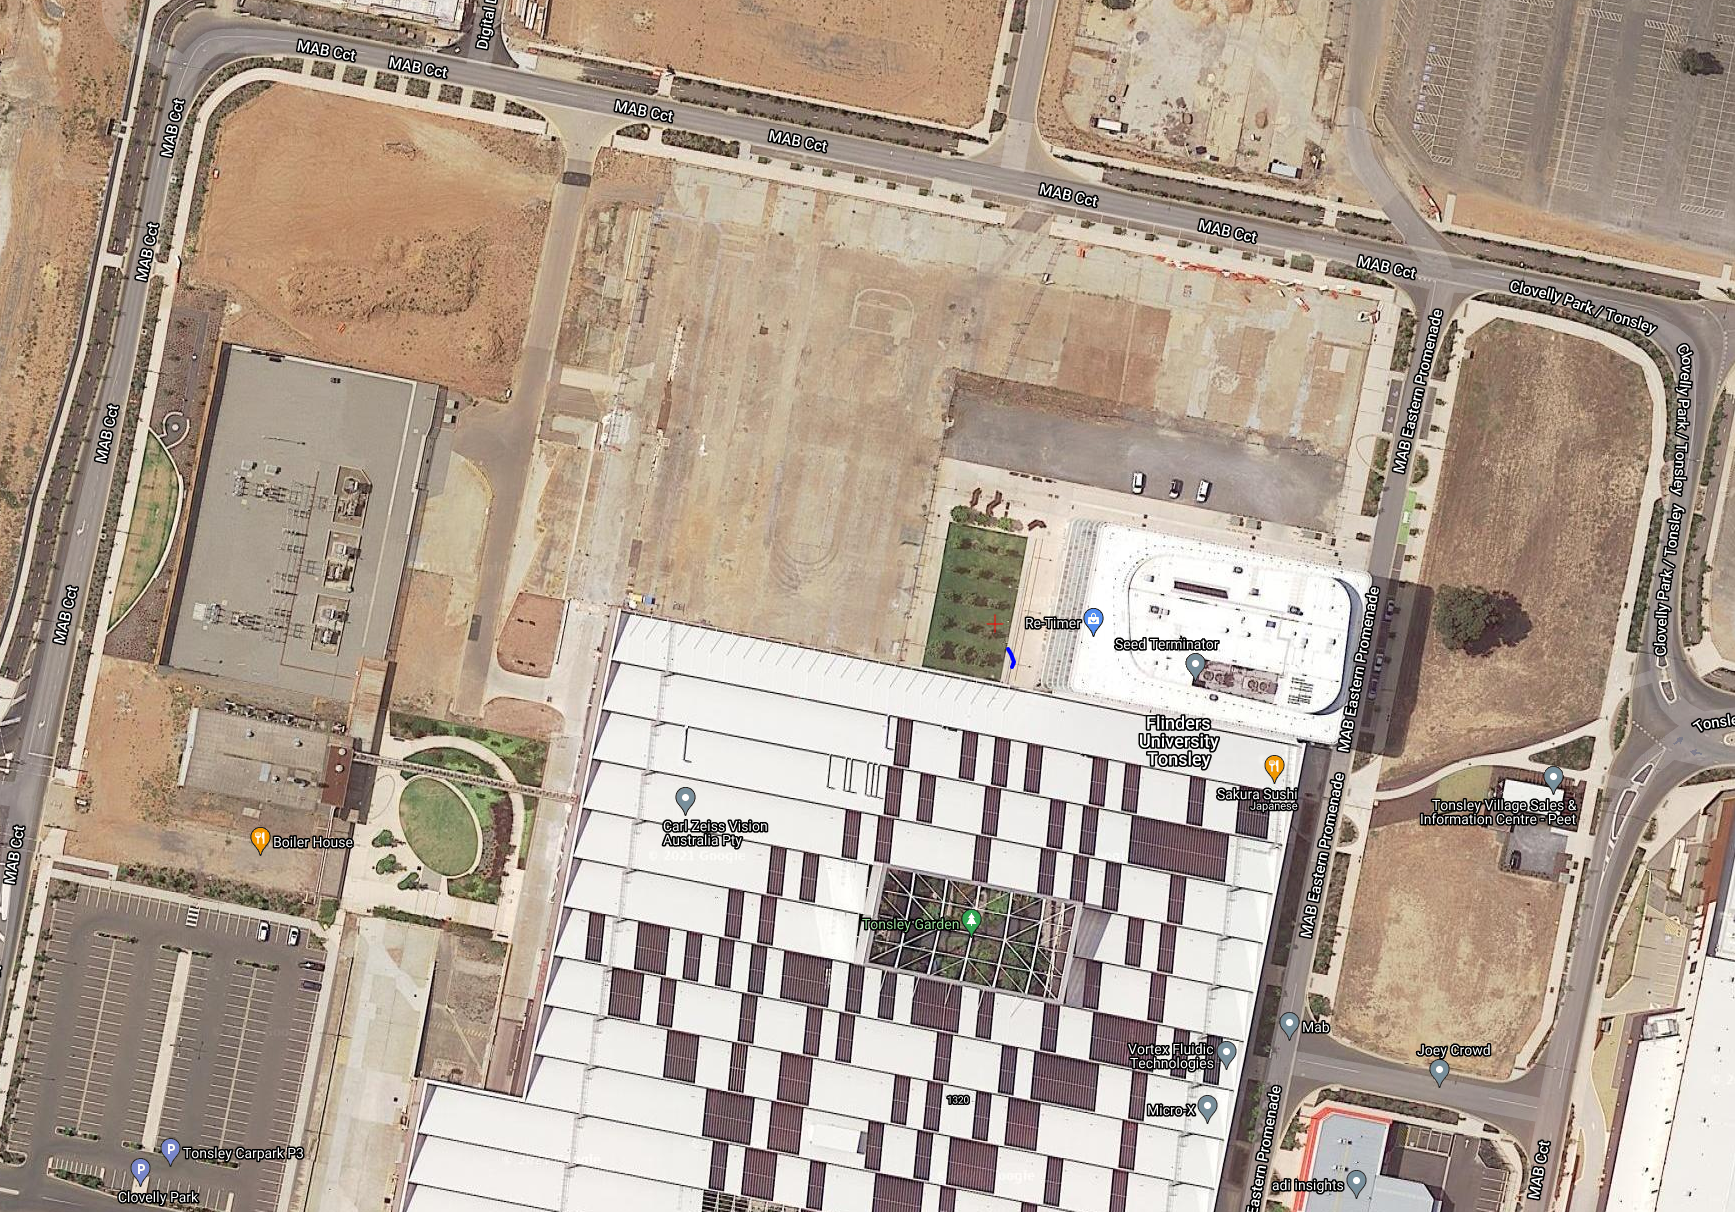
\includegraphics[width=14cm,keepaspectratio]{Figures/2021_3_30_static_MAB_Satellite.PNG}
        \caption{Satellite image with expected GPS position shown with red cross and recorded position shown with blue line}
        \label{fig:MABSatelliteImage}
    \end{centering}
\end{figure}

\subsubsection{Antarctica}
Davis station in Antarctica was chosen as a location for spoofing. As mentioned above the coordinates for this location was $-68.5762449235, 77.9696166515$. The COTS
receiver was used as a spoof victim and it was successfully spoofed. Figure \ref{fig:antarcticaStaticCNo} shows the carrier to noise graph over the spoof attack. There is
a consistent value of $\approx 50 dBHz$ plus signals that are consistently at $\approx 40 dBHz$. Time to first fix was shown to be approximately 60 seconds, this is the
lower end of the fix times from experiments for cold starts. It can be see that there is consistent signals for the first 50 seconds. For the time pereiod between 70 and
200 seconds there was more volatile signal quality. Figure \ref{fig:antarcticaStaticError} shows that there was a high, but consistent level of error between first fix
and 140 seconds. After this there was a spike, which is associated with a drop of lock, and the high error remained until the end of the test. This high error is evident
when viewing the raw position in Figure \ref{fig:antarcticaStaticCoord} and with respect to the desired location, Figure \ref{fig:antarcticaStaticPosition}. Figure \ref{fig:antarcticaSatelliteImage} shows this error
in position in more context placed over a satellite image.
The inaccuracy is higher than was expected from this experiment.  

\begin{figure}[!h]
    \begin{centering}
        \includegraphics[width=14cm,keepaspectratio]{Figures/2021_3_30_static_antarctica Carrier noise ratio.png}
        \caption{Carrier to noise ratio from unique SVIDs as broadcast by SDR and received by GPS receiver at Davis Station in Antarctica on 30th March 2021. Each SVID has been given a unique colour.}
        \label{fig:antarcticaStaticCNo}
    \end{centering}
\end{figure}

\begin{figure}[!h]
    \begin{centering}
        \includegraphics[width=14cm,keepaspectratio]{Figures/2021_3_30_static_antarctica Lat long position.png}
        \caption{Trace of latitude and longitude over time as interpreted from the GPS receiver with expected location noted with red dot}
        \label{fig:antarcticaStaticCoord}
    \end{centering}
\end{figure}

\begin{figure}[!h]
    \begin{centering}
        \includegraphics[width=14cm,keepaspectratio]{Figures/2021_3_30_static_antarctica Position from origin.png}
        \caption{Graph of recorded position with respect to the intended spoofed location}
        \label{fig:antarcticaStaticPosition}
    \end{centering}
\end{figure}

\begin{figure}[!h]
    \begin{centering}
        \includegraphics[width=14cm,keepaspectratio]{Figures/2021_3_30_static_antarctica error over time.png}
        \caption{Error between calculated location and expected location over time}
        \label{fig:antarcticaStaticError}
    \end{centering}
\end{figure}

\begin{figure}[!h]
    \begin{centering}
        \includegraphics[width=14cm,keepaspectratio]{Figures/2021_3_30_static_antarctica_Satellite.PNG}
        \caption{Satellite image with expected GPS position shown with red cross and recorded position shown with blue line}
        \label{fig:antarcticaSatelliteImage}
    \end{centering}
\end{figure}

\subsection{Dynamic Spoofing}

\subsubsection{Tonsley MAB}
The time to first fix was shown to be approximately 49 seconds.


\begin{figure}[h]
    \begin{centering}
        \includegraphics[width=14cm,keepaspectratio]{Figures/2021_3_30_dynamic_MAB Carrier noise ratio.png}
        \caption{Carrier to noise ratio from unique SVIDs as broadcast by SDR and received by GPS receiver at MAB in Tonsley on 30th March 2021. Each SVID has been given a unique colour.}
        \label{fig:MABdynamicCNo}
    \end{centering}
\end{figure}

\begin{figure}[h]
    \begin{centering}
        \includegraphics[width=14cm,keepaspectratio]{Figures/2021_3_30_dynamic_MAB Lat long position.png}
        \caption{Trace of latitude and longitude over time as interpreted from the GPS receiver with expected location noted with red dot}
        \label{fig:MABdynamicCoord}
    \end{centering}
\end{figure}

\begin{figure}[h]
    \begin{centering}
        \includegraphics[width=14cm,keepaspectratio]{Figures/2021_3_30_dynamic_MAB Position from origin.png}
        \caption{Graph of recorded position with respect to the intended spoofed location}
        \label{fig:MABdynamicPosition}
    \end{centering}
\end{figure}

\begin{figure}[h]
    \begin{centering}
        \includegraphics[width=14cm,keepaspectratio]{Figures/2021_3_30_dynamic_MAB_Satellite.PNG}
        \caption{Satellite image with expected GPS position shown with red cross and recorded position shown with blue line}
        \label{fig:MABdynamicSatelliteImage}
    \end{centering}
\end{figure}

\subsection{Issues Encountered}
The under run issue was more or less solved by increasing the buffer size to $40\times$ greater than the sampling size.
There was an issue towards the end of the project where there was considerable leakage of EM radiation into the Faraday cage that was causing the GPS receiver to produce
wildly inaccurate position (up to and over 500m error). This was much different to what had previously been recorded within the Faraday cage. This amount of error does
not constitute a successful spoof since the time to first lock was much greater than a real signal, or even spoofing attempts previously. 

During initial testing of the spoofing there was an inability to get the spoofer to correctly spoof the receiver. It was found that there is a requirement that the ratio
between the sampling frequency and clock frequency of the radio must be an integer value. Therefore when compiling the signal using GPS-SDR-sim the sampling frequency
value was required to be changed to 2.5Msps.  

Just after the testing phase of the project the smartphone that was being used for some of the logging and graphing was rendered unusable. While there was no data lost,
it was replaced with a newer model that experimentally was much harder to spoof than the previous model. This could be due to many factors including anti-spoofing
algorithms \cite{RN39}. It would be a fair assessment that the newer device is able to receive more GNSS signals including augmented systems as well as other signals such as Wi-Fi.
The connection to the Wi-Fi signal was such that notifications were coming up on the phone while performing the experiments.

There were a number of unterminated cables that were running from outside of the cage to inside. This was seen as being the cause of the issues that were being faced. The
suspect cables were removed or terminated and the results were more consistent with what was being achieved previously. Even with the new phone the GPS location was able
to be spoofed.

From sources \todo{insert source} it was found that the SVID and PRN are the same thing. 
A common result from spoofed attempts was to have GPS satellites with an SVID of over 100. GPS satellites have PRN codes from 1-63 and augmentation systems have PRNs from
64 to 158 \cite{RN67}. From the list of PRN codes \cite{RN67} it can be seen that the services that are being received are some kind of augmented system. \emph{This makes
me think that there might be a GBAS system or SBAS system nearby that is being received within the cage by stray wires etc.}

\section{Experimental Issues}
While performing experiments there were issues that were run into that were required to be overcome. Initially a Log Periodic antenna was used for transmission since its
frequency range was appropriate for use transmitting L1 band signals. After experiments failed to pick up any signals it was swapped for a omnidirectional antenna. This
was able to produce signals that were picked up by the GNSS Logger application. Observing the graphs of the carrier to noise figure showed that when there was an under run
issue the $\frac{C}{N_0}$ would drop to 0 and the GPS receiver in the phone would lose connection to the 'satellites'. This meant that no GPS lock was achievable.  

In an attempt to overcome the under run issue that was plaguing the experiments, a new PC was brought in with Ubuntu installed directly instead of via a VM. This resulted
in the radio working straight away. The under run issues resurfaced when trying to read the serial data from a COTS GPS receiver. This was less than ideal and required a
second computer to act as a datalogger.
